\documentclass[aspectratio=169,10pt]{beamer}
\usepackage[utf8]{inputenc}
\usepackage[T1]{fontenc}
\usepackage{booktabs,graphicx,amsmath}
\usetheme{default}
\usecolortheme{seahorse}
\setbeamertemplate{navigation symbols}{}
\setbeamertemplate{footline}[frame number]
\setbeamerfont{frametitle}{size=\large}

\begin{document}

% ---------------------------------------------------------------- slide 1
\begin{frame}{Trigger hybride warp + additif (+ photométrique) : protocole et variantes testées}
\small
\textbf{Trigger} : $x' = \mathrm{clamp}\big(\,\mathrm{photo}(\mathrm{warp}(x)) + \delta,\,0,1\big)$, optimisé conjointement
(grille de warp $k\times k$ bornée par \texttt{warp\_s}~px, $\|\delta\|_\infty\le\epsilon$, et, optionnellement, contraste $1{+}a_c$ et luminosité $b_c$ par canal).

\medskip
\textbf{Protocole} : r32p / CIFAR-10, camion$\to$cerf, \textbf{une seule seed}, génération avec agrégateur \texttt{mean}.
Déploiement sur 8 budgets de labels retournés $\{0,\dots,5000\}$ : \emph{centralisé} (mean, 1 empoisonné)
et \emph{fédéré} multikrum 3 vs 7. Mesure : ASR final.

\medskip
\centering
\scriptsize
\setlength{\tabcolsep}{3pt}
\begin{tabular}{@{}llcccc@{\hspace{8pt}}l@{}}
\toprule
& Variante & \multicolumn{2}{c}{ASR multikrum (\%)} & \multicolumn{2}{c}{ASR centralisé (\%)} & Visibilité \\
\cmidrule(lr){3-4}\cmidrule(lr){5-6}
& & budget 0 & 5000 & budget 0 & 5000 & \\
\midrule
A & $\epsilon{=}0.3$, warp 8\,px ($k{=}4$)            & 78 & 88 & 18 & 98  & images méconnaissables \\
B & $\epsilon{=}0.0627$, warp 8\,px ($k{=}4$)         & 13 & 41 & 24 & 97  & images méconnaissables \\
C & $\epsilon{=}0.0627$, warp 2\,px ($k{=}8$)         & 12 & 50 & 22 & 96  & déformation nette, rayures \\
D & C + photo $\pm0.1$ / $\pm0.03$                      & \textbf{65} & 74 & \textbf{72} & 98 & déformation nette + assombri \\
E & $\epsilon{=}0.05$, warp 1.5\,px, photo $\pm0.05$ / $\pm0.015$ & 15 & 9 & 5 & 100 & déformation encore visible \\
\bottomrule
\end{tabular}

\medskip
\raggedright
\footnotesize
\vspace{-1mm}
Le budget~0 (aucun label retourné) sert de \textbf{ligne de base} : un ASR élevé à budget~0 signale un trigger qui agit comme une perturbation adverse sur le modèle propre, pas un backdoor appris.
\end{frame}

% ---------------------------------------------------------------- slide 2
\begin{frame}{Résultats : ASR en fonction du budget, et enseignements}
\centering
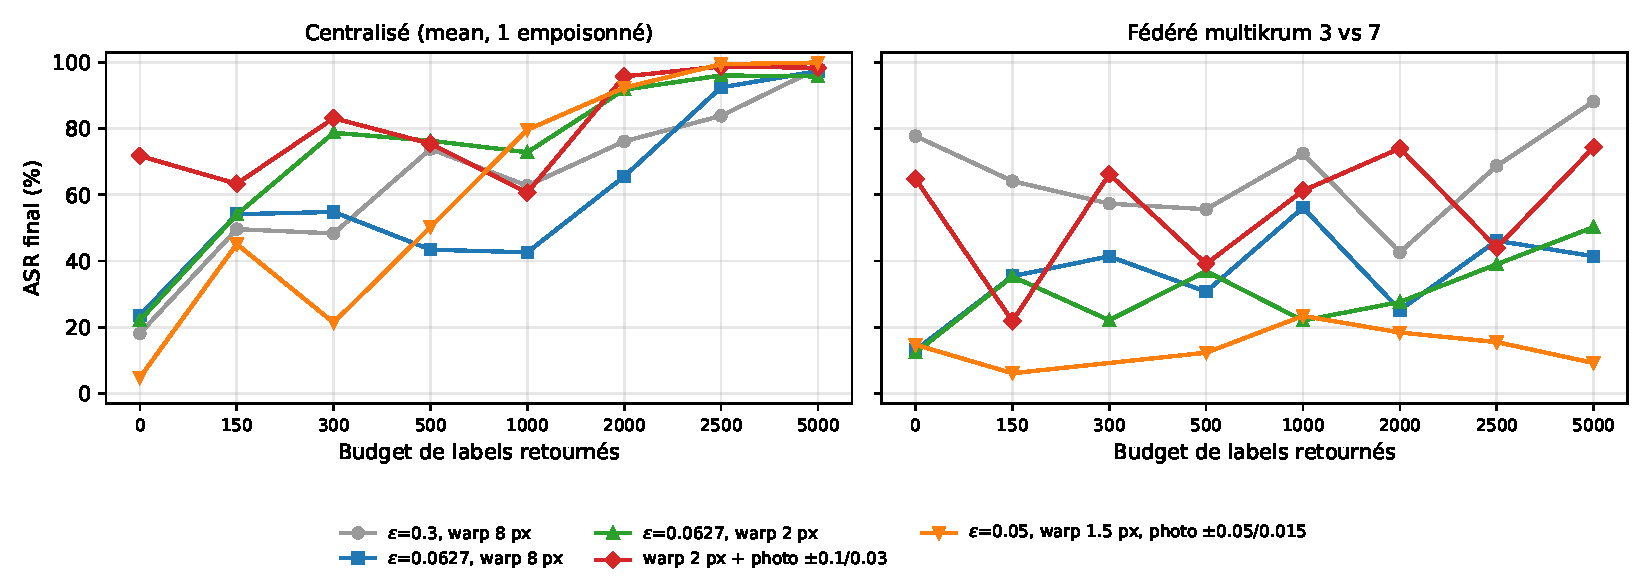
\includegraphics[width=0.84\textwidth]{asr_vs_budget_hybrid.pdf}

\vspace{-2mm}
\raggedright
\scriptsize
\begin{itemize}\setlength{\itemsep}{1pt}
  \item \textbf{Effet adverse} : $\epsilon{=}0.3$ (A) et la photométrie large (D) donnent 65--78\,\% d'ASR \emph{sans aucun label retourné} : l'ASR brut n'y mesure pas un backdoor.
  \item \textbf{Warp 8$\to$2\,px} (B$\to$C, $\epsilon$ fixé) : backdoor mieux appris en centralisé (79\,\% contre 55\,\% à 300 labels), mais pas de gain face à multikrum (50\,\% contre 41\,\% à 5000).
  \item \textbf{Contraintes serrées} (E) : ASR de base 5\,\% / 15\,\%, centralisé 100\,\% à 5000, mais multikrum le bloque ($\le$\,23\,\%) : la déformation du warp reste visible sur des images texturées, et le trigger ne franchit pas l'agrégateur.
  \item \textbf{Limites} : une seule seed (écarts fédérés de l'ordre du bruit) ; point E fédéré à 300 labels manquant (erreur CUDA sur une machine, non relancé).
  \item \textbf{Suite envisagée} : warp 1.5\,px avec photométrie $\pm0.1$ / $\pm0.03$.
\end{itemize}
\end{frame}

% ---------------------------------------------------------------- slide 3
\begin{frame}{Les triggers testés, appliqués aux mêmes images}
\centering
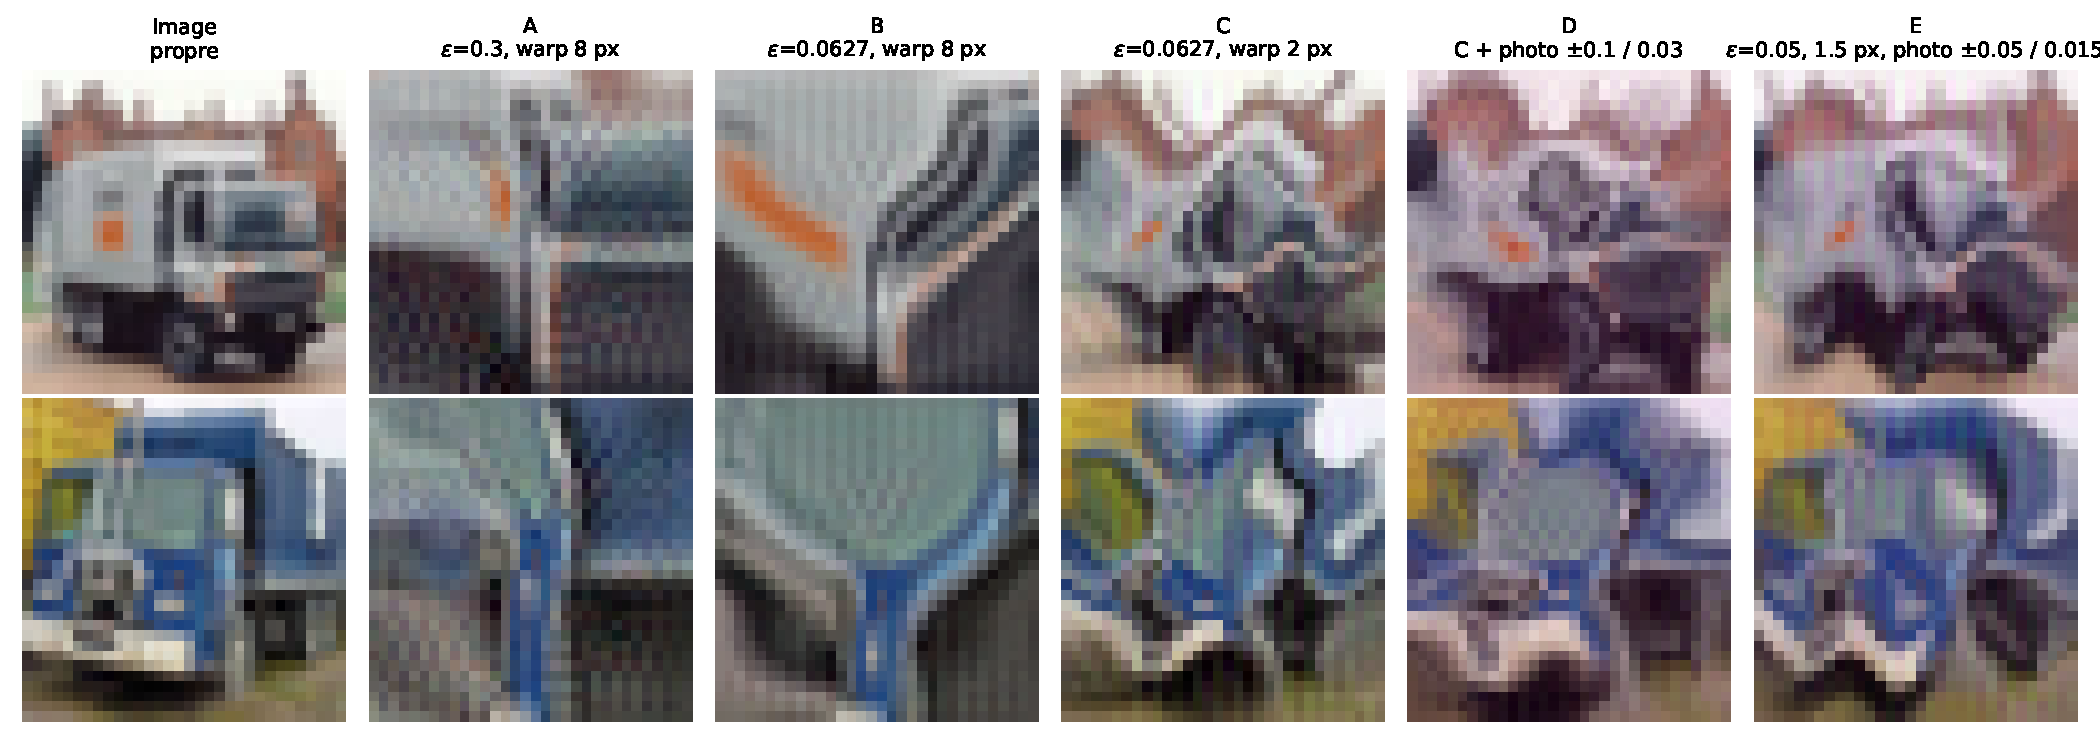
\includegraphics[width=0.93\textwidth,height=0.66\textheight,keepaspectratio]{triggers_comparison_slide.pdf}

\vspace{-1mm}
\raggedright
\scriptsize
\begin{itemize}\setlength{\itemsep}{1pt}
  \item La grille de warp est \emph{indépendante de l'image} : la même déformation s'applique à tous les camions.
  \item A et B (8\,px) rendent les images méconnaissables ; C, D et E (2\,px et moins) restent nettement déformées (roues, contours), avec des rayures verticales dues à $\delta$.
  \item C'est le warp, plus que $\delta$ ou la photométrie, qui fixe la visibilité : un trigger discret demanderait un \texttt{warp\_s} bien plus petit (non testé).
\end{itemize}
\end{frame}

\end{document}
